\documentclass[8pt,aspectratio=169]{beamer}
\usetheme{Madrid}
\usepackage{graphicx}
\usepackage{booktabs}
\usepackage{adjustbox}
\usepackage{multicol}
\usepackage{amsmath}
\usepackage{amssymb}
\usepackage{listings}
\usepackage{array}
\usepackage{tikz}
\usetikzlibrary{positioning,shapes.geometric}

% Colours of pca_efa_komplett.tex, the house look
\definecolor{mlblue}{RGB}{0,102,204}
\definecolor{mlpurple}{RGB}{51,51,178}
\definecolor{mllavender}{RGB}{173,173,224}
\definecolor{mllavender2}{RGB}{193,193,232}
\definecolor{mllavender3}{RGB}{204,204,235}
\definecolor{mllavender4}{RGB}{214,214,239}
\definecolor{mlorange}{RGB}{255, 127, 14}
\definecolor{mlgreen}{RGB}{44, 160, 44}
\definecolor{mlred}{RGB}{214, 39, 40}
\definecolor{mlgray}{RGB}{127, 127, 127}

% Additional colors
\definecolor{lightgray}{RGB}{240, 240, 240}
\definecolor{midgray}{RGB}{180, 180, 180}

% Apply custom colors to Madrid theme
\setbeamercolor{palette primary}{bg=mllavender3,fg=mlpurple}
\setbeamercolor{palette secondary}{bg=mllavender2,fg=mlpurple}
\setbeamercolor{palette tertiary}{bg=mllavender,fg=white}
\setbeamercolor{palette quaternary}{bg=mlpurple,fg=white}

\setbeamercolor{structure}{fg=mlpurple}
\setbeamercolor{section in toc}{fg=mlpurple}
\setbeamercolor{subsection in toc}{fg=mlblue}
\setbeamercolor{title}{fg=mlpurple}
\setbeamercolor{frametitle}{fg=mlpurple,bg=mllavender3}
\setbeamercolor{block title}{bg=mllavender2,fg=mlpurple}
\setbeamercolor{block body}{bg=mllavender4,fg=black}

% Remove navigation symbols
\setbeamertemplate{navigation symbols}{}

% Clean itemize/enumerate
\setbeamertemplate{itemize items}[circle]
\setbeamertemplate{enumerate items}[default]

% Reduce margins
\setbeamersize{text margin left=5mm,text margin right=5mm}

% Bottom note command
\newcommand{\bottomnote}[1]{%
\vfill\vspace{-2mm}
\textcolor{mllavender2}{\rule{\textwidth}{0.4pt}}
\vspace{1mm}\footnotesize\textbf{#1}}

% Compact list spacing
\newcommand{\compactlist}{%
\setlength{\itemsep}{0pt}%
\setlength{\parskip}{0pt}%
\setlength{\parsep}{0pt}}

% R code listings
\lstset{
  language=R,
  basicstyle=\tiny\ttfamily,
  keywordstyle=\color{mlblue},
  commentstyle=\color{mlgray}\itshape,
  stringstyle=\color{mlpurple},
  numbers=left,
  numberstyle=\tiny\color{mlgray},
  backgroundcolor=\color{lightgray},
  frame=single,
  frameround=tttt,
  rulecolor=\color{mllavender2},
  breaklines=true,
  showstringspaces=false,
  escapeinside={\%*}{*)}
}


% ================================================================ house-lecture
% \lecturepart{k}{name}{goal}: part k of the lecture, its name (the \section
% title, the contents-page title, the footline) and its one learning goal.
% \contentslist{k}: every part; parts before k grey with a check and no goal,
% part k in mlorange with its goal, later parts with their goals. Each name is
% a link to the part's contents page, a frame with label=partk.
\newcounter{lpparts}
\newcommand{\lecturepart}[3]{%
  \expandafter\gdef\csname lpname#1\endcsname{#2}%
  \expandafter\gdef\csname lpgoal#1\endcsname{#3}%
  \ifnum#1>\value{lpparts}\setcounter{lpparts}{#1}\fi}
\newcommand{\lpname}[1]{\csname lpname#1\endcsname}
\newcommand{\lpgoal}[1]{\csname lpgoal#1\endcsname}
\newcommand{\contentsrow}[2]{%
  \ifnum#2<#1
    {\large\color{mlgray}\makebox[1.6em][l]{$\checkmark$}\makebox[1.3em][l]{#2}\hyperlink{part#2}{\lpname{#2}}\par}%
  \else\ifnum#2=#1
    {\large\bfseries\color{mlorange}\makebox[1.6em][l]{$\blacktriangleright$}\makebox[1.3em][l]{#2}\hyperlink{part#2}{\lpname{#2}}\par}%
    {\leftskip=2.9em\color{mlorange}\lpgoal{#2}\par}%
  \else
    {\large\makebox[1.6em][l]{}\makebox[1.3em][l]{#2}\hyperlink{part#2}{\lpname{#2}}\par}%
    {\leftskip=2.9em\color{black!75}\lpgoal{#2}\par}%
  \fi\fi
  \vspace{0.45em}}
\newcommand{\contentslist}[1]{%
  \vspace{0.8em}%
  \foreach \lpn in {1,...,\thelpparts}{\contentsrow{#1}{\lpn}}%
  \vspace{0.3em}%
  {\small\color{mlgray}\ifnum#1>1 $\checkmark$~finished\quad\fi
   {\color{mlorange}$\blacktriangleright$}~next\quad
   under each part ahead: its learning goal\par}}

% Footline: Madrid's three boxes, the current part's name in the middle one,
% the short title before the first part.
\makeatletter
\newcommand{\partortitle}{\ifx\insertsectionhead\@empty\insertshorttitle\else\insertsectionhead\fi}
\makeatother
\setbeamertemplate{footline}{%
  \leavevmode%
  \hbox{%
  \begin{beamercolorbox}[wd=.333333\paperwidth,ht=2.25ex,dp=1ex,center]{author in head/foot}%
    \usebeamerfont{author in head/foot}\insertshortauthor
  \end{beamercolorbox}%
  \begin{beamercolorbox}[wd=.333333\paperwidth,ht=2.25ex,dp=1ex,center]{title in head/foot}%
    \usebeamerfont{title in head/foot}\partortitle
  \end{beamercolorbox}%
  \begin{beamercolorbox}[wd=.333333\paperwidth,ht=2.25ex,dp=1ex,right]{date in head/foot}%
    \usebeamerfont{date in head/foot}\insertframenumber{} / \inserttotalframenumber\hspace*{2ex}
  \end{beamercolorbox}}%
  \vskip0pt}

% The parts of this lecture: name, one learning goal each.
\lecturepart{1}{Next-Token Distribution}{Compute next-token probabilities from scores; write the probability of a continuation as a product.}
\lecturepart{2}{Greedy Decoding}{Name the greedy token; explain the repetition loop.}
\lecturepart{3}{Temperature}{Name the limits of $p^{(T)}$ as $T \to 0$, $T \to \infty$.}
\lecturepart{4}{Top-k, Top-p}{Choose top-$k$ or top-$p$ for a peaked or a flat distribution.}
\lecturepart{5}{Beam Search}{Run beam search of width $B$ on a two-step tree.}
\lecturepart{6}{Worked Example: GPT-2 Small}{Compute each rule on the numbers of GPT-2 small after one prompt.}

% The five rules between the distribution p and the next token: part 1, takeaways.
\newcommand{\decodingdiagram}{%
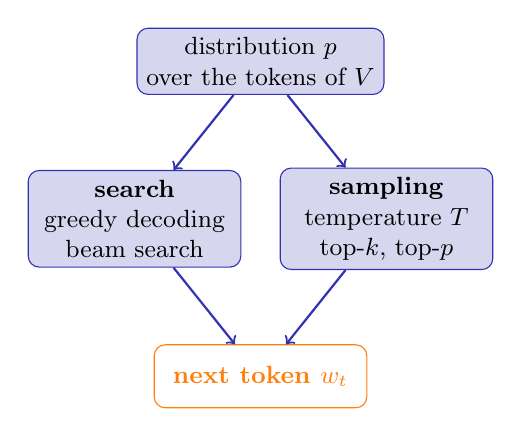
\begin{tikzpicture}[
  box/.style={rectangle, rounded corners, draw=mlpurple, fill=mllavender4, align=center, font=\small, minimum width=2.7cm, minimum height=0.8cm},
  arr/.style={->, thick, mlpurple}]
  \node[box] (p) at (0, 0) {distribution $p$\\over the tokens of $V$};
  \node[box] (s) at (-1.6, -2.0) {\textbf{search}\\greedy decoding\\beam search};
  \node[box] (d) at (1.6, -2.0) {\textbf{sampling}\\temperature $T$\\top-$k$, top-$p$};
  \node[box, draw=mlorange, fill=white, text=mlorange, font=\small\bfseries] (w) at (0, -4.0) {next token $w_t$};
  \draw[arr] (p) -- (s);
  \draw[arr] (p) -- (d);
  \draw[arr] (s) -- (w);
  \draw[arr] (d) -- (w);
\end{tikzpicture}}

\newcommand{\colab}[1]{https://colab.research.google.com/github/josterri/teaching-nlp-notebooks-sampling/blob/main/#1.ipynb}

\title[Picking the Next Token]{Picking the Next Token,\\Greedy Decoding to Beam Search}
\subtitle{Text Analytics, Chapter 7}
\author[J.~Osterrieder]{Prof.\ Dr.\ J\"org Osterrieder}
\institute[]{}
\date{}

\begin{document}

% ==================== TITLE ====================
\begin{frame}[plain]
\titlepage
\end{frame}

% ==================== HOOK ====================
\begin{frame}[t]{One Prompt, Two Continuations}
\begin{columns}[T]
\column{0.48\textwidth}
\textbf{Scenario:} You send one prompt to a chatbot twice and receive two different continuations.

\vspace{3mm}
\begin{itemize}\compactlist
\item After the prompt, the language model has a probability $p_i$ for each token $i$ of its vocabulary $V$
\item One token is appended, and the step is repeated on the longer text
\item With a random draw at each step, two runs give two texts
\item The question: which token is appended, under which rule
\end{itemize}

\column{0.48\textwidth}
\begin{center}
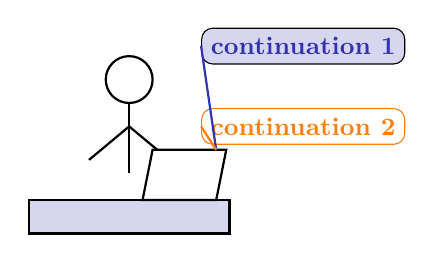
\begin{tikzpicture}[scale=0.85]
  \draw[thick, fill=mllavender4] (-1.5,-0.5) rectangle (1.5,0);
  \draw[thick] (0,1.8) circle (0.35);
  \draw[thick] (0,1.45) -- (0,0.4);
  \draw[thick] (0,1.1) -- (-0.6,0.6);
  \draw[thick] (0,1.1) -- (0.6,0.6);
  \draw[thick, fill=white] (0.2,0) -- (1.3,0) -- (1.45,0.75) -- (0.35,0.75) -- cycle;
  \node[draw, rounded corners, fill=mllavender4, text=mlpurple, font=\small\bfseries] (c1) at (2.6,2.3) {continuation 1};
  \node[draw, rounded corners, fill=white, text=mlorange, draw=mlorange, font=\small\bfseries] (c2) at (2.6,1.1) {continuation 2};
  \draw[thick, mlpurple] (1.3,0.75) -- (c1.west);
  \draw[thick, mlorange] (1.3,0.75) -- (c2.west);
\end{tikzpicture}
\end{center}
\end{columns}

\bottomnote{The appended token depends on the decoding rule.}
\note{2 min. Ask who has received two different answers to one question from a chatbot. Both answers come from one distribution per step; the difference lies in the rule by which the token is picked. Five rules are compared: greedy decoding, temperature, top-k, top-p, beam search.}
\end{frame}

% ==================== CONTENTS 1 ====================
% no-bottomnote: the parts, part 1 next, the learning goals ahead.
\begin{frame}[t,label=part1]{Learning Goals for Decoding}
\contentslist{1}
\vspace{0.2em}
{\color{mlgray}Worked Example: GPT-2 small after the first words of \textit{Pride and Prejudice}.\par}
\note{0.5 min. Read the six learning goals aloud, part 1 first. Parts 1 to 5 are in symbols and schematic charts; every number of GPT-2 small is in part 6.}
\end{frame}

\section{Next-Token Distribution}

% ==================== CONCEPT: SOFTMAX ====================
\begin{frame}[t]{Softmax Probabilities From Scores}
\begin{columns}[T]
\column{0.48\textwidth}
\begin{block}{Definition}
After a context $c$, the language model has a \textbf{score} $z_i$ for each token $i$ of the vocabulary $V$. The \textbf{softmax} of the scores is the next-token probability
\[ p_i = \frac{e^{z_i}}{\sum_{j \in V} e^{z_j}}. \]
\end{block}

\vspace{1mm}
\textbf{Intuition:}
\begin{itemize}\compactlist
\item A larger score $\rightarrow$ a larger probability
\item $p_i > 0$ for every token, $\sum_i p_i = 1$
\item $z_i + a$ for every token $\rightarrow$ the same $p$: only differences of scores count
\end{itemize}

\column{0.48\textwidth}
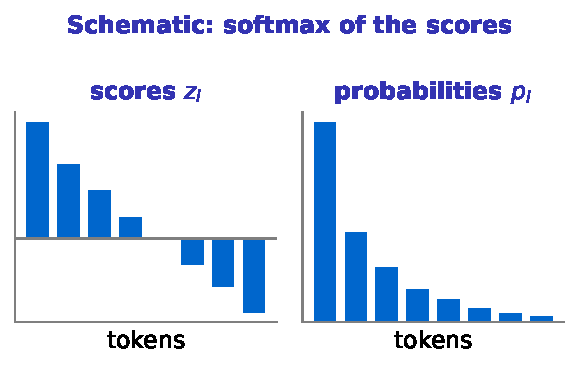
\includegraphics[width=\textwidth]{images/softmax_scores.pdf}
\end{columns}

\bottomnote{The softmax of the scores is the next-token distribution $p$.}
\note{2 min. Point at the negative scores in the left panel: each has a positive probability in the right one. Ask the room what happens to $p$ when a constant $a$ is added to every score: nothing, since $e^{z_i + a} = e^{a} e^{z_i}$ and $e^{a}$ cancels. A token is a word or a piece of a word.}
\end{frame}

% ==================== CONCEPT: PRODUCT ====================
\begin{frame}[t]{Probability of a Continuation as a Product}
\begin{columns}[T]
\column{0.48\textwidth}
\begin{block}{Definition}
A \textbf{continuation} $w_1, \dots, w_n$ of the context $c$ has the probability
\[ P = \prod_{t=1}^{n} p(w_t \mid c, w_{<t}), \quad \log P = \sum_{t=1}^{n} \log p(w_t \mid c, w_{<t}). \]
\end{block}

\vspace{1mm}
\textbf{Intuition:}
\begin{itemize}\compactlist
\item Each factor is at most 1 $\rightarrow$ $P$ falls with every token
\item $\log P \le 0$; closer to 0 $\rightarrow$ a more probable continuation
\item A large first factor can be followed by small ones
\end{itemize}

\column{0.48\textwidth}
\begin{center}
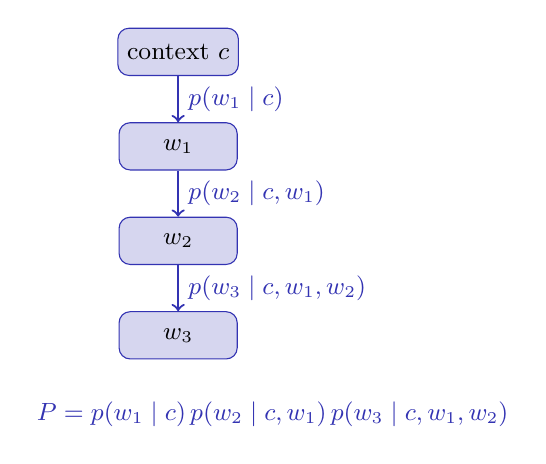
\begin{tikzpicture}[
  tk/.style={rectangle, rounded corners, draw=mlpurple, fill=mllavender4, font=\small, minimum width=1.5cm, minimum height=0.6cm},
  arr/.style={->, thick, mlpurple}]
  \node[tk] (c) at (0, 0) {context $c$};
  \node[tk] (w1) at (0, -1.2) {$w_1$};
  \node[tk] (w2) at (0, -2.4) {$w_2$};
  \node[tk] (w3) at (0, -3.6) {$w_3$};
  \draw[arr] (c) -- node[right, font=\small] {$p(w_1 \mid c)$} (w1);
  \draw[arr] (w1) -- node[right, font=\small] {$p(w_2 \mid c, w_1)$} (w2);
  \draw[arr] (w2) -- node[right, font=\small] {$p(w_3 \mid c, w_1, w_2)$} (w3);
  \node[font=\small, text=mlpurple] at (1.2, -4.6) {$P = p(w_1 \mid c)\, p(w_2 \mid c, w_1)\, p(w_3 \mid c, w_1, w_2)$};
\end{tikzpicture}
\end{center}
\end{columns}

\bottomnote{The probability of a continuation is the product of its next-token probabilities.}
\note{2 min. Each factor is a softmax probability after a longer context: the context grows by one token per step. Ask why $\log P$ is used: a product of many small numbers underflows in floating point, a sum of logarithms stays in range. The first factor alone gives little information on $P$; part 5 has a case.}
\end{frame}

% ==================== CONCEPT: RULES ====================
\begin{frame}[t]{Decoding Rules: Search, Sampling}
\begin{columns}[T]
\column{0.48\textwidth}
\begin{block}{Definition}
A \textbf{decoding rule} is a map from the distribution $p$ at a step to the next token: by a \textbf{search} for a probable continuation, or by a \textbf{draw} from a distribution $q$ derived from $p$.
\end{block}

\vspace{1mm}
\begin{itemize}\compactlist
\item Search: greedy decoding, beam search $\rightarrow$ one text for one prompt
\item Sampling: temperature $T$, top-$k$, top-$p$ $\rightarrow$ a new text on each run
\item Temperature first, then a cut by top-$k$ or top-$p$: the sampling rules are combined
\end{itemize}

\column{0.48\textwidth}
\begin{center}
\decodingdiagram
\end{center}
\end{columns}

\bottomnote{Under search, one prompt gives one text; under sampling, each run gives a new text.}
\note{2 min. Ask the room which kind is behind the two answers of the scenario: sampling. In machine translation, beam search is the common rule, since one output is wanted. The four rules of sampling share one step: a draw from $q$.}
\end{frame}

\section{Greedy Decoding}

% ==================== CONTENTS 2 ====================
% no-bottomnote: the parts, part 2 next, the learning goals ahead.
\begin{frame}[t,label=part2]{Greedy Decoding}
\contentslist{2}
\note{0.5 min. Read goal 2 aloud. Greedy decoding is the rule with no parameter and no draw.}
\end{frame}

% ==================== CONCEPT: GREEDY ====================
\begin{frame}[t]{The Greedy Token Has the Largest Probability}
\begin{columns}[T]
\column{0.48\textwidth}
\begin{block}{Definition}
Under \textbf{greedy decoding}, the next token is the token with the largest probability, at every step:
\[ w_t = \arg\max_{i \in V}\, p(i \mid c, w_{<t}). \]
\end{block}

\vspace{1mm}
\textbf{Intuition:}
\begin{itemize}\compactlist
\item No draw $\rightarrow$ one prompt, one text, on every run
\item Each step is decided alone: later probabilities stay out of the comparison
\item Greedy decoding is temperature at $T \to 0$ and beam search at $B = 1$
\end{itemize}

\column{0.48\textwidth}
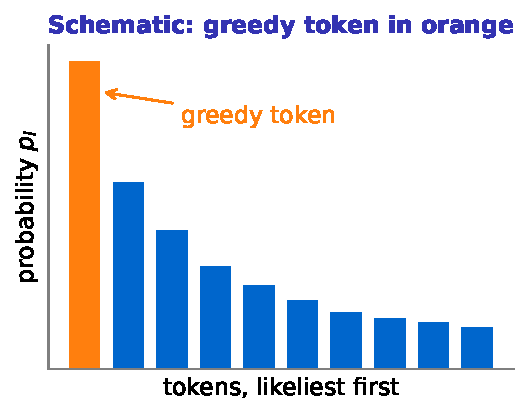
\includegraphics[width=\textwidth]{images/greedy_bars.pdf}
\end{columns}

\bottomnote{Under greedy decoding, the likeliest token is appended at every step.}
\note{2 min. Ask the room to run greedy decoding twice in their heads: the same text both times. The orange bar is the appended token. The most probable token at each step can differ from the most probable continuation; the beam search part has the condition.}
\end{frame}

% ==================== DISCOVERY REVEAL: LOOP ====================
\begin{frame}[t]{Probability of a Repeated Phrase}
\begin{columns}[T]
\column{0.48\textwidth}
Under greedy decoding, a text can end in a loop: one phrase, repeated again and again.

\vspace{3mm}
\begin{block}{Discovery}
Each copy of the phrase is added to the context. With every copy, does the probability of the next copy grow or fall?

\uncover<2->{\textbf{Answer:} it grows. With each copy in the context, the next copy has a larger probability, and the loop continues to the last token (Holtzman et al., 2020).}
\end{block}

\column{0.48\textwidth}
\only<1>{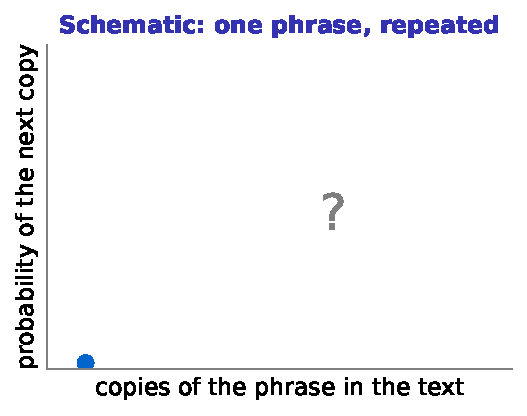
\includegraphics[width=\textwidth]{images/repeat_q.pdf}}%
\only<2>{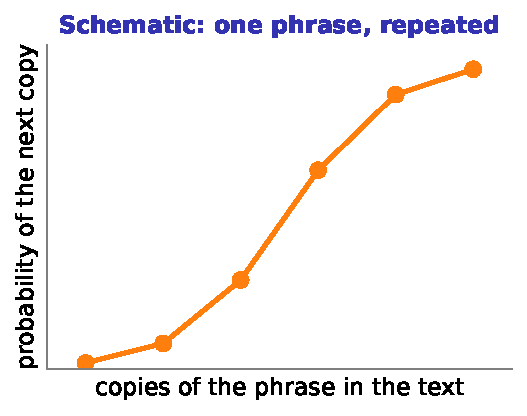
\includegraphics[width=\textwidth]{images/repeat_a.pdf}}
\end{columns}

\bottomnote{Under greedy decoding, the probability of a repeated phrase grows with each copy.}
\note{2.5 min. Give the room one minute. Holtzman et al. (2020) found the rise for most phrases they tested with GPT-2. Under greedy decoding the loop has no exit: after a copy, the likeliest token is the start of the next copy. Part 6 has six copies of one sentence after one prompt.}
\end{frame}

\section{Temperature}

% ==================== CONTENTS 3 ====================
% no-bottomnote: the parts, part 3 next, the learning goals ahead.
\begin{frame}[t,label=part3]{Temperature}
\contentslist{3}
\note{0.5 min. Read goal 3 aloud. With temperature, the first rule of sampling, a token is drawn at random.}
\end{frame}

% ==================== CONCEPT: TEMPERATURE ====================
\begin{frame}[t]{Scores Divided by T Before the Softmax}
\begin{columns}[T]
\column{0.48\textwidth}
\begin{block}{Definition}
Under \textbf{sampling}, the next token is drawn at random from a distribution $q$. With \textbf{temperature} $T > 0$, $q = p^{(T)}$:
\[ p_i^{(T)} = \frac{e^{z_i / T}}{\sum_{j \in V} e^{z_j / T}}. \]
\end{block}

\vspace{1mm}
\textbf{Intuition:}
\begin{itemize}\compactlist
\item $T < 1$ $\rightarrow$ more mass on the likeliest tokens
\item $T > 1$ $\rightarrow$ the mass spread over more tokens
\item The order of the tokens is the same at every $T$; $T = 1$ gives $p$
\end{itemize}

\column{0.48\textwidth}
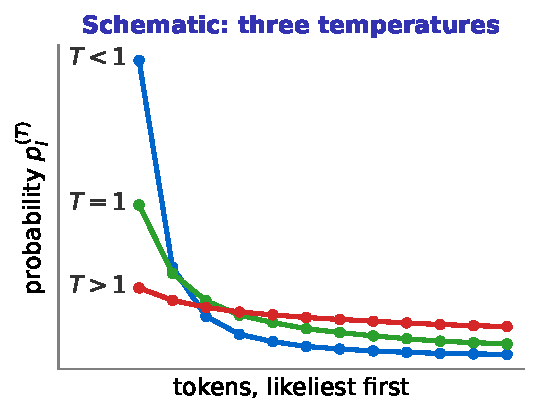
\includegraphics[width=\textwidth]{images/temperature_three.pdf}
\end{columns}

\bottomnote{Under temperature $T$, the scores are divided by $T$ before the softmax.}
\note{2 min. Ask why the order is the same: division by a positive $T$ keeps $z_i > z_j$. The ratio of two probabilities is $p_i^{(T)} / p_j^{(T)} = e^{(z_i - z_j)/T}$: below $T = 1$ it is larger than at $T = 1$, above $T = 1$ closer to 1.}
\end{frame}

% ==================== DISCOVERY REVEAL: LIMITS ====================
\begin{frame}[t]{Two Limits of the Temperature}
\begin{columns}[T]
\column{0.48\textwidth}
Temperature $T$ in the softmax: $p_i^{(T)} \propto e^{z_i / T}$, with two limits.

\vspace{3mm}
\begin{block}{Discovery}
Which distribution is $p^{(T)}$ as $T \to 0$, which as $T \to \infty$?

\uncover<2->{\textbf{Answer:} $T \to 0$: all mass on the largest score, so a draw from $p^{(T)}$ equals greedy decoding. $T \to \infty$: $z_i / T \to 0$ for every token, so $p_i^{(T)} \to 1/|V|$, the uniform distribution.}
\end{block}

\column{0.48\textwidth}
\only<1>{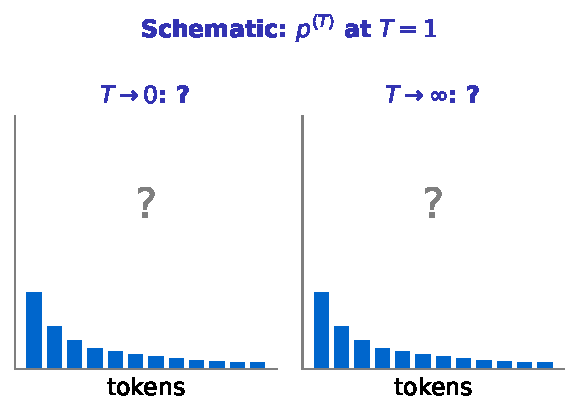
\includegraphics[width=\textwidth]{images/limits_q.pdf}}%
\only<2>{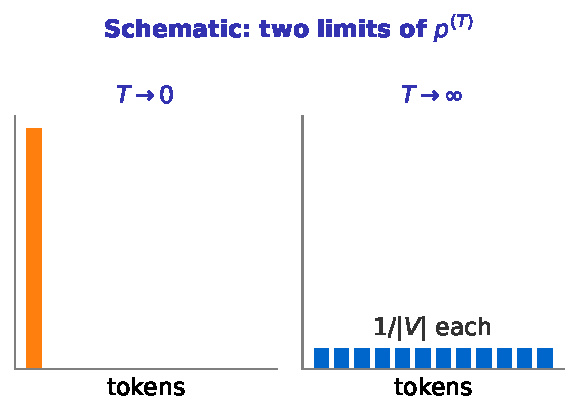
\includegraphics[width=\textwidth]{images/limits_a.pdf}}
\end{columns}

\bottomnote{At $T \to 0$, sampling equals greedy decoding; at $T \to \infty$, every token has probability $1/|V|$.}
\note{2.5 min. One minute for the room. For $T \to 0$: the ratio $e^{(z_{\max} - z_i)/T}$ grows without bound for every other token. For $T \to \infty$, a draw is a token picked uniformly at random, and the text is a list of unrelated tokens.}
\end{frame}

% ==================== CONCEPT: ENTROPY ====================
\begin{frame}[t]{Entropy Grows With Temperature}
\begin{columns}[T]
\column{0.48\textwidth}
\begin{block}{Definition}
The \textbf{entropy} of a distribution $p$ is $H(p) = -\sum_i p_i \log p_i$, in nats. $H = 0$ when one token has all the mass; $H = \log |V|$ under the uniform distribution.
\end{block}

\vspace{1mm}
\textbf{Intuition:}
\begin{itemize}\compactlist
\item $\dfrac{dH}{dT} = \dfrac{\mathrm{Var}_{p^{(T)}}(z)}{T^3} \ge 0$ (Appendix A2)
\item $H$ grows with $T$, from 0 to $\log |V|$
\item A larger $H$ $\rightarrow$ a less predictable next token
\end{itemize}

\column{0.48\textwidth}
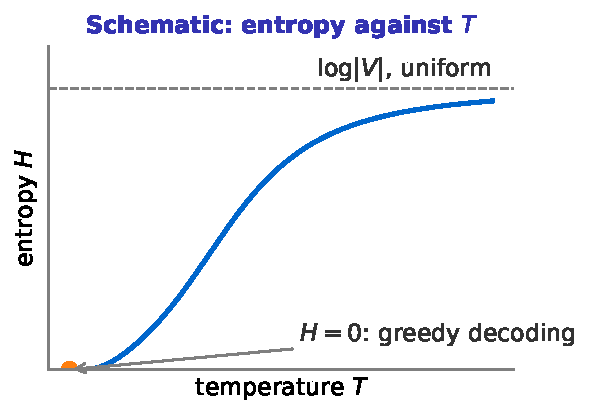
\includegraphics[width=\textwidth]{images/entropy_T.pdf}
\end{columns}

\bottomnote{The entropy of $p^{(T)}$ grows with the temperature, from 0 to $\log |V|$.}
\note{2 min. $e^{H}$ is the number of equally likely tokens with the same entropy: at $H = \log |V|$ it is $|V|$. The numerator of the derivative is the variance of the scores under $p^{(T)}$, so the derivative is zero only when all scores are equal.}
\end{frame}

\section{Top-k, Top-p}

% ==================== CONTENTS 4 ====================
% no-bottomnote: the parts, part 4 next, the learning goals ahead.
\begin{frame}[t,label=part4]{Top-k, Top-p}
\contentslist{4}
\note{0.5 min. Read goal 4 aloud. Top-k, top-p are cuts: the unlikely tokens are removed before the draw.}
\end{frame}

% ==================== CONCEPT: TOP-K ====================
\begin{frame}[t]{Top-k: the k Likeliest Tokens}
\begin{columns}[T]
\column{0.48\textwidth}
\begin{block}{Definition}
Under \textbf{top-k} sampling, the set $S_k$ of the $k$ likeliest tokens is kept, with the mass $M_k = \sum_{i \in S_k} p_i$. The draw is from
\[ q_i = p_i / M_k \ \ (i \in S_k), \qquad q_i = 0 \ \text{otherwise}. \]
\end{block}

\vspace{1mm}
\textbf{Intuition:}
\begin{itemize}\compactlist
\item The number of kept tokens is fixed at $k$
\item The kept mass $M_k$ depends on $p$
\item $k = 1$ $\rightarrow$ greedy decoding; $k = |V|$ $\rightarrow$ $p$ itself
\end{itemize}

\column{0.48\textwidth}
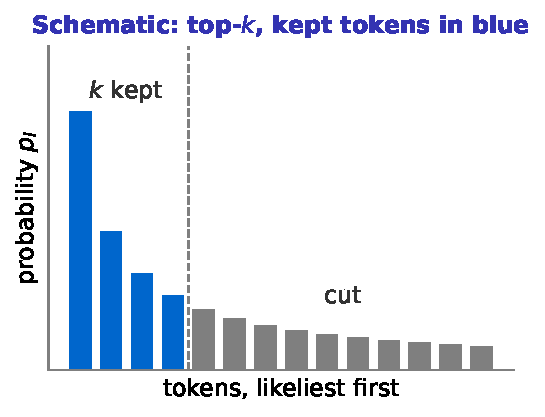
\includegraphics[width=\textwidth]{images/topk_cut.pdf}
\end{columns}

\bottomnote{Under top-$k$, the $k$ likeliest tokens are kept, whatever their mass.}
\note{2 min. Ask what is lost: the mass $1 - M_k$ of the cut tokens. The divergence of $q$ from $p$ is $\mathrm{KL}(q \parallel p) = -\log M_k$ (Appendix A3). Fan et al. (2018) introduced top-k sampling for story generation.}
\end{frame}

% ==================== CONCEPT: TOP-P ====================
\begin{frame}[t]{Top-p: the Smallest Set With Mass $\pi$}
\begin{columns}[T]
\column{0.48\textwidth}
\begin{block}{Definition}
Under \textbf{top-p} sampling, or nucleus sampling, the kept set is the smallest set of likeliest tokens with mass $M \ge \pi$. The draw is from $q_i = p_i / M$ on that set; its size is $k^*(\pi)$.
\end{block}

\vspace{1mm}
\textbf{Intuition:}
\begin{itemize}\compactlist
\item The kept mass is fixed: $M \ge \pi$
\item The number of kept tokens $k^*(\pi)$ depends on $p$
\item $\pi \to 0$ $\rightarrow$ greedy decoding; $\pi = 1$ $\rightarrow$ $p$ itself
\end{itemize}

\column{0.48\textwidth}
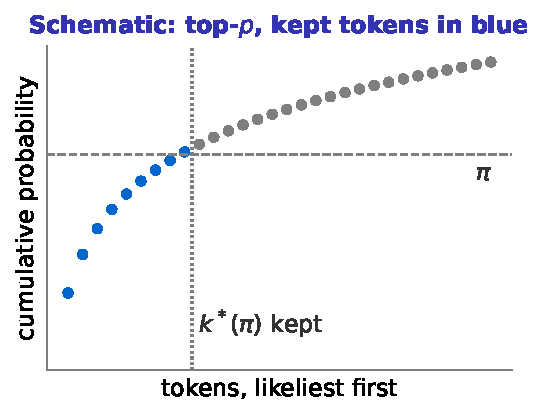
\includegraphics[width=\textwidth]{images/topp_cum.pdf}
\end{columns}

\bottomnote{Under top-$p$, the likeliest tokens are kept until their mass is at least $\pi$.}
\note{2 min. Holtzman et al. (2020) introduced nucleus sampling. Ask how many tokens are kept when one token alone has a mass above $\pi$: one, and the draw is greedy decoding. The bound $\mathrm{KL}(q \parallel p) \le -\log \pi$ holds after every prompt (Appendix A3).}
\end{frame}

% ==================== DISCOVERY REVEAL: PEAKED, FLAT ====================
\begin{frame}[t]{Fixed k Against Fixed $\pi$ on Two Distributions}
\begin{columns}[T]
\column{0.48\textwidth}
Two distributions: a peaked one, with most of the mass on one token; a flat one, with the mass spread over many tokens.

\vspace{3mm}
\begin{block}{Discovery}
One $k$, one $\pi$ for both. Under top-$k$, after which distribution is the cut mass $1 - M_k$ larger? Under top-$p$, after which are more tokens kept?

\uncover<2->{\textbf{Answer:} the flat one, both times. Under top-$k$, most of its mass is cut, and almost none of the peaked one. Under top-$p$, the kept mass is at least $\pi$ after both, with many tokens of the flat one, few of the peaked one.}
\end{block}

\column{0.48\textwidth}
\only<1>{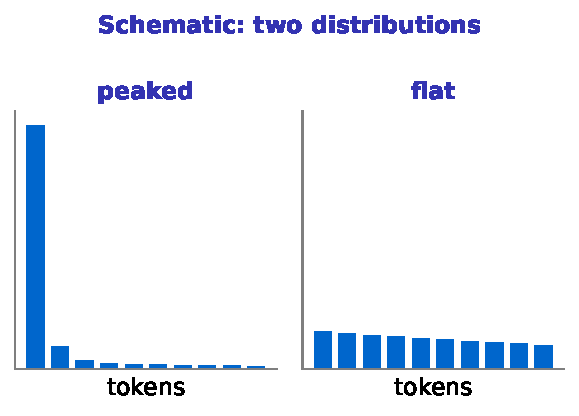
\includegraphics[width=\textwidth]{images/twodist_q.pdf}}%
\only<2>{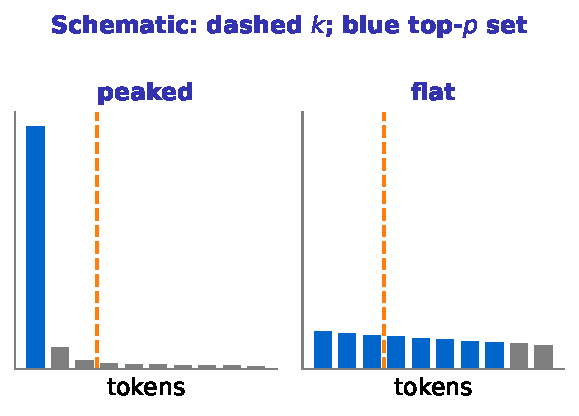
\includegraphics[width=\textwidth]{images/twodist_a.pdf}}
\end{columns}

\bottomnote{Under top-$k$ the number of kept tokens is fixed; under top-$p$, the kept mass.}
\note{2.5 min. One minute for the room. In the second chart, the dashed line marks $k$. With one $k$, tokens of near-zero probability are kept after the peaked distribution, and likely tokens are cut after the flat one. Part 6 has the numbers of GPT-2 small after a peaked, a flat prompt.}
\end{frame}

\section{Beam Search}

% ==================== CONTENTS 5 ====================
% no-bottomnote: the parts, part 5 next, the learning goals ahead.
\begin{frame}[t,label=part5]{Beam Search}
\contentslist{5}
\note{0.5 min. Read goal 5 aloud. Beam search is the second search rule: several partial continuations are compared at each step.}
\end{frame}

% ==================== STEPS ====================
\begin{frame}[t]{Beam Search of Width B in Four Steps}
\begin{block}{Definition}
Under \textbf{beam search} of width $B$, the $B$ partial continuations with the largest $\log P$ are kept at every step; the result has the largest $\log P$ at the end.
\end{block}

\vspace{2mm}
\textbf{The four steps:}
\begin{enumerate}\compactlist
\item \textbf{Start} with the context $c$ as one partial continuation, $\log P = 0$
\item \textbf{Extend} each kept partial continuation by every token $i$: $\log P + \log p(i \mid \cdot)$
\item \textbf{Keep} the $B$ largest of the $B \cdot |V|$ extensions
\item \textbf{Repeat} steps 2, 3 until $n$ tokens are appended
\end{enumerate}

\vspace{3mm}
\begin{block}{Discovery}
At $B = 1$, which decoding rule is beam search?
\pause

Greedy decoding: one partial continuation, extended by its likeliest token.
\end{block}

\bottomnote{Beam search of width 1 is greedy decoding.}
\note{3 min. Write the four steps on the board as a loop. At each step, $B \cdot |V|$ extensions are compared, against $|V|$ under greedy decoding. Ask the room for the answer before the second step. Beam search is a search: one prompt gives one text on every run.}
\end{frame}

% ==================== DISCOVERY REVEAL: TREE ====================
\begin{frame}[t]{Greedy Path Against the Most Probable Path}
\begin{columns}[T]
\column{0.48\textwidth}
Two first tokens $a$, $b$ with $p_a > p_b$. After $a$, the mass is spread over many tokens; after $b$, most of it is on one token $y$.

\vspace{3mm}
\begin{block}{Discovery}
Under which condition is the path $b\,y$ more probable than every path starting with $a$?

\uncover<2->{\textbf{Answer:} when $p_b\, p(y \mid b) > p_a \max_x p(x \mid a)$. Under greedy decoding, $b$ is dropped at the first step. Under beam search with $B \ge 2$, $b$ is kept, and $b\,y$ is the result.}
\end{block}

\column{0.48\textwidth}
\begin{center}
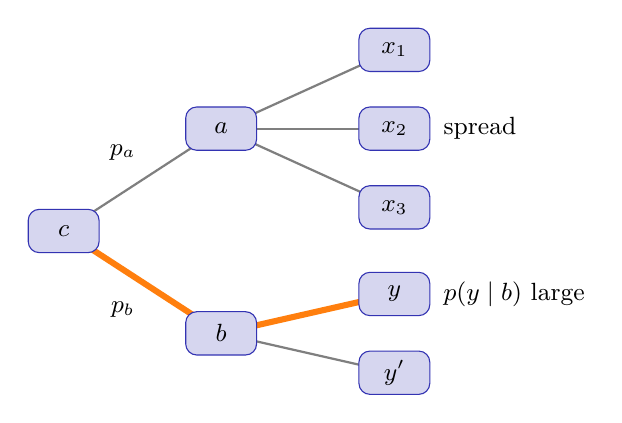
\begin{tikzpicture}[
  tk/.style={rectangle, rounded corners, draw=mlpurple, fill=mllavender4, font=\small, minimum width=0.9cm, minimum height=0.55cm},
  ed/.style={thick, mlgray}]
  \coordinate (c) at (0, 0);
  \coordinate (a) at (2.0, 1.3);
  \coordinate (b) at (2.0, -1.3);
  \draw[ed] (c) -- (a);
  \draw[ed] (c) -- (b);
  \foreach \y in {2.3, 1.3, 0.3} \draw[ed] (a) -- (4.2, \y);
  \draw[ed] (b) -- (4.2, -0.8);
  \draw[ed] (b) -- (4.2, -1.8);
  \only<2>{\draw[mlorange, line width=2.2pt] (c) -- (b) -- (4.2, -0.8);}
  \node[tk] at (c) {$c$};
  \node[tk] at (a) {$a$};
  \node[tk] at (b) {$b$};
  \node[font=\small] at (0.75, 1.0) {$p_a$};
  \node[font=\small] at (0.75, -1.0) {$p_b$};
  \foreach \y/\l in {2.3/x_1, 1.3/x_2, 0.3/x_3} \node[tk] at (4.2, \y) {$\l$};
  \node[tk] at (4.2, -0.8) {$y$};
  \node[tk] at (4.2, -1.8) {$y'$};
  \node[font=\small, anchor=west] at (4.7, 1.3) {spread};
  \node[font=\small, anchor=west] at (4.7, -0.8) {$p(y \mid b)$ large};
\end{tikzpicture}
\end{center}
\end{columns}

\bottomnote{A first token of smaller probability can begin the most probable continuation.}
\note{2.5 min. One minute for the room. The condition has two sides: the first factor of $a$ is larger, the second factor of $b$ is larger. Ask for the smallest $B$ with $b\,y$ as the result: $B = 2$, since $b$ is the second likeliest first token. Part 6 has the case with the numbers of GPT-2 small.}
\end{frame}

% ==================== CHECKPOINT QUIZ ====================
\begin{frame}[t]{Checkpoint: Beam Width, Search Result}
\begin{block}{Checkpoint problem}
Beam search of width $B$ over $V$, $n$ steps after a context $c$.
\end{block}

\vspace{3mm}
\textbf{Question 1:} For $n = 2$, which smallest $B$ gives the most probable two-token continuation after every context?
\pause

\vspace{1mm}
\textbf{Answer:} $\mathbf{B = |V|}$: every first token is kept, all $|V|^2$ paths are compared. With a smaller $B$, the best path can start with a dropped token.

\vspace{3mm}
\textbf{Question 2:} At the end, which is larger: $\log P$ at width $B$, or $\log P$ at width $B + 1$?
\pause

\vspace{1mm}
\textbf{Answer:} \textbf{either one}: at width $B + 1$, another set can be kept at an intermediate step, without the result of width $B$.

\bottomnote{With a wider beam, more paths are compared, and the result can have a smaller $\log P$.}
\note{3 min. One minute per question. For question 1, the worst case: the most probable path starts with the least likely first token. For question 2, part 6 has $\log P$ at $B = 1$ above $\log P$ at $B = 2$ after one prompt. An exact search over $n$ steps has $|V|^n$ paths.}
\end{frame}

% ==================== COMPARISON ====================
\begin{frame}[t]{Five Decoding Rules in Six Aspects}
Six aspects of the five decoding rules, at one step:

\vspace{2mm}
\begin{center}
\begin{tabular}{llllll}
\toprule
Aspect & Greedy & Temperature & Top-$k$ & Top-$p$ & Beam search \\
\midrule
Kind & search & sampling & sampling & sampling & search \\
Parameter & none & $T$ & $k$ & $\pi$ & $B$ \\
One text per prompt & yes & no & no & no & yes \\
Kept at a step & 1 token & all of $V$ & $k$ tokens & $k^*(\pi)$ tokens & $B$ paths \\
Number kept depends on $p$ & no & no & no & yes & no \\
Equal to greedy decoding at & every setting & $T \to 0$ & $k = 1$ & $\pi \to 0$ & $B = 1$ \\
\bottomrule
\end{tabular}
\end{center}

\bottomnote{Greedy decoding is a limit of each of the four other rules.}
\note{2 min. Read the last row: each rule has a setting equal to greedy decoding. The sampling rules are chained: temperature first, then top-k or top-p, as in Hugging Face transformers. Ask which row separates top-k from top-p: the number kept.}
\end{frame}

% ==================== DECISION FLOWCHART ====================
\begin{frame}[t]{From the Task to a Decoding Rule}
\begin{center}
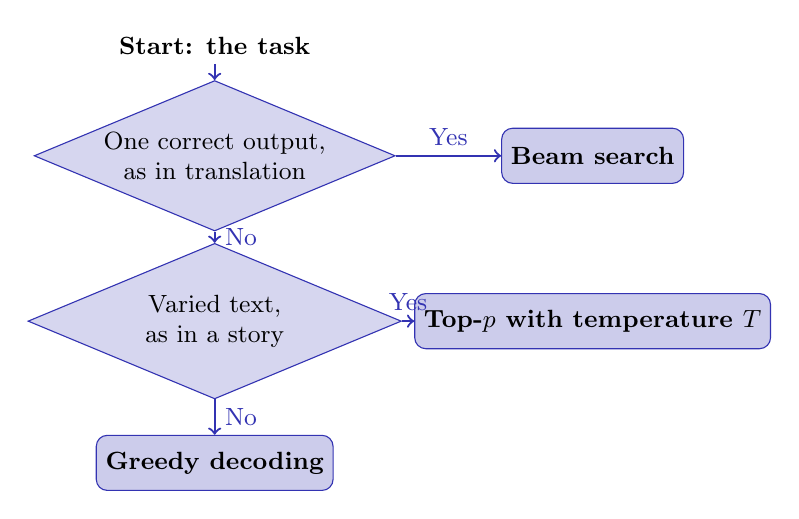
\begin{tikzpicture}[
  dec/.style={diamond, draw=mlpurple, fill=mllavender4, aspect=2.4, inner sep=1pt, align=center, font=\small, text width=2.9cm, execute at begin node={\hyphenpenalty=10000}},
  res/.style={rectangle, rounded corners, draw=mlpurple, fill=mllavender3, align=center, font=\small\bfseries, minimum width=2.2cm, minimum height=0.7cm},
  arr/.style={->, thick, mlpurple}]
  \node[font=\small\bfseries] (start) at (0, 0) {Start: the task};
  \node[dec] (q1) at (0, -1.4) {One correct output, as in translation};
  \node[res] (beam) at (4.8, -1.4) {Beam search};
  \node[dec] (q2) at (0, -3.5) {Varied text, as in a story};
  \node[res] (topp) at (4.8, -3.5) {Top-$p$ with temperature $T$};
  \node[res] (greedy) at (0, -5.3) {Greedy decoding};
  \draw[arr] (start) -- (q1);
  \draw[arr] (q1) -- node[above, font=\small] {Yes} (beam);
  \draw[arr] (q1) -- node[right, font=\small] {No} (q2);
  \draw[arr] (q2) -- node[above, font=\small] {Yes} (topp);
  \draw[arr] (q2) -- node[right, font=\small] {No} (greedy);
\end{tikzpicture}
\end{center}

\bottomnote{The decoding rule is chosen from the task, before any text is generated.}
\note{2 min. Put two tasks to the room: a German sentence into English, with beam search; a bedtime story told twice, with top-p and a temperature, so that each run differs. A quick test of a prompt, with one text: greedy decoding.}
\end{frame}

\section{Worked Example: GPT-2 Small}

% ==================== CONTENTS 6 ====================
% no-bottomnote: the parts, part 6 next, the learning goals ahead.
\begin{frame}[t,label=part6]{Worked Example: GPT-2 Small}
\contentslist{6}
\note{0.5 min. Read goal 6 aloud. Every number in part 6 is computed by GPT-2 small after three prompts; the three Colab notebooks have the same numbers.}
\end{frame}

% ==================== WORKED NUMBERS: TOKENS ====================
\begin{frame}[t]{Ten Likeliest Tokens After the Austen Prompt}
\begin{columns}[T]
\column{0.48\textwidth}
\begin{block}{Definition}
The \textbf{Austen prompt} is the context \textit{It is a truth universally acknowledged that}, the first words of \textit{Pride and Prejudice} (1813). GPT-2 small has $|V| = 50{,}257$ tokens.
\end{block}

\vspace{1mm}
\textbf{Worked:} the five likeliest next tokens at $T = 1$:

\vspace{1mm}
\begin{tabular}{lrr}
\toprule
Token & Score $z_i$ & $p_i$ \\
\midrule
\texttt{the} & $-87.547$ & 0.182 \\
\texttt{there} & $-89.120$ & 0.038 \\
\texttt{a} & $-89.514$ & 0.025 \\
\texttt{we} & $-89.788$ & 0.019 \\
\texttt{in} & $-90.090$ & 0.014 \\
\midrule
Five tokens & & 0.278 \\
\bottomrule
\end{tabular}

\vspace{1mm}
\textbf{Worked:} greedy decoding gives \texttt{the}; under top-$p$ with $\pi = 0.9$, 3{,}784 tokens are kept.

\column{0.48\textwidth}
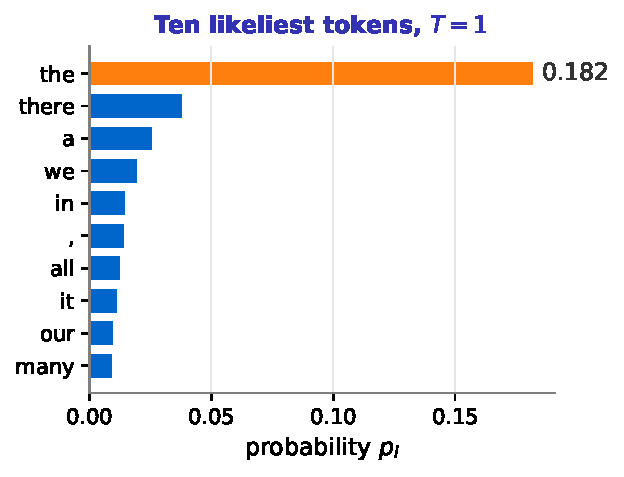
\includegraphics[width=\textwidth]{images/austen_top10.pdf}
\end{columns}

\bottomnote{After the Austen prompt, the likeliest token has probability 0.182, and 3,784 tokens have a mass of 0.9.}
\note{1.5 min. The scores are near $-90$; only their differences count. Add the column on the board: $0.182 + 0.038 + 0.025 + 0.019 + 0.014 = 0.278$. Under greedy decoding, \texttt{the} is appended. With 3,784 tokens for 0.9 of the mass, the distribution after this prompt is flat.}
\end{frame}

% ==================== COMPUTATION IN TWO COLUMNS ====================
\begin{frame}[t]{Ratio of the Two Likeliest Tokens at T = 0.5, 1, 2}
\begin{columns}[T]
\column{0.48\textwidth}
\textbf{Step 1:} the scores of the two likeliest tokens after the Austen prompt

\vspace{2mm}
\begin{tabular}{lr}
\toprule
Token & Score $z_i$ \\
\midrule
\texttt{the} & $-87.547$ \\
\texttt{there} & $-89.120$ \\
\midrule
$\Delta = z_{\text{the}} - z_{\text{there}}$ & 1.573 \\
\bottomrule
\end{tabular}

\vspace{2mm}
Under temperature $T$, the ratio is $p^{(T)}_{\text{the}} / p^{(T)}_{\text{there}} = e^{\Delta / T}$.

\column{0.48\textwidth}
\textbf{Step 2:} the ratio at three temperatures
\[ e^{1.573/0.5} = 23.2, \quad e^{1.573/1} = 4.82, \quad e^{1.573/2} = 2.20 \]

\textbf{Reading the results:}
\begin{itemize}\compactlist
\item $p_{\text{the}} = 0.885$ at $T = 0.5$, $0.182$ at $T = 1$, $0.005$ at $T = 2$
\item $H = 0.69$, $6.38$, $9.88$ nats, against $\log |V| = 10.82$
\item At every $T$, \texttt{the} is the likeliest token
\end{itemize}
\end{columns}

\bottomnote{At $T = 0.5$, \texttt{the} is 23.2 times as probable as \texttt{there}; at $T = 2$, 2.20 times.}
\note{2 min. Compute $e^{3.146}$ on the board: 23.2. For the ratio, two scores suffice; for $p_{\text{the}}$ itself, all 50,257, since the denominator of the softmax is a sum over the vocabulary. The entropies show the limits of part 3: 0.69 nats is near greedy decoding, 9.88 near the uniform 10.82.}
\end{frame}

% ==================== WORKED NUMBERS: TOP-K, TOP-P ====================
\begin{frame}[t]{Top-k Mass, Top-p Size After Three Prompts}
\begin{columns}[T]
\column{0.48\textwidth}
\begin{block}{Definition}
The \textbf{peaked prompt} is \textit{The Prime Minister of the United}; the \textbf{flat prompt} is \textit{I went to the}.
\end{block}

\vspace{1mm}
\textbf{Worked:} three prompts, top-$k$ mass $M_5$, top-$p$ size $k^*(0.9)$:

\vspace{1mm}
\begin{tabular}{lrrr}
\toprule
Prompt & $p_{\max}$ & Mass $M_5$ & Size $k^*(0.9)$ \\
\midrule
peaked & 0.799 & 0.992 & 2 \\
Austen & 0.182 & 0.278 & 3{,}784 \\
flat & 0.033 & 0.112 & 4{,}797 \\
\bottomrule
\end{tabular}

\vspace{2mm}
\textbf{Worked:} under top-k with $k = 5$ after the flat prompt, \texttt{hospital} has $q = 0.033 / 0.112 = 0.295$; under top-p, 4{,}797 tokens are kept.

\column{0.48\textwidth}
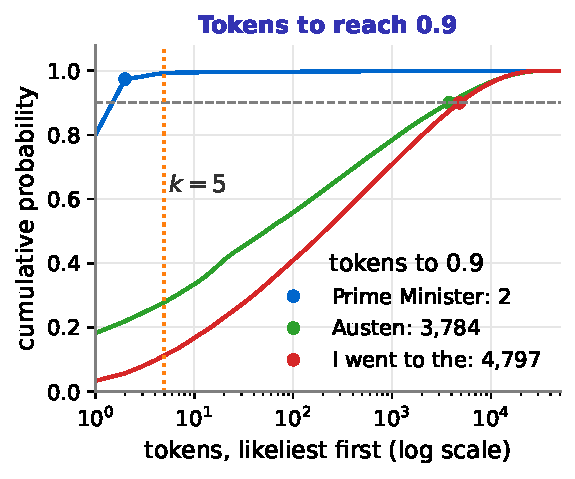
\includegraphics[width=\textwidth]{images/cumulative_three.pdf}
\end{columns}

\bottomnote{At $k = 5$, 0.992 of the mass is kept after the peaked prompt, 0.112 after the flat one.}
\note{2 min. Read the table by columns: $M_5$ from 0.992 to 0.112, $k^*(0.9)$ from 2 to 4,797. The divergence of top-5 is $-\log 0.112 = 2.19$ nats after the flat prompt, $-\log 0.992 = 0.008$ after the peaked one. In the chart, $k = 5$ is the dotted line, 0.9 the dashed one.}
\end{frame}

% ==================== WORKED NUMBERS: TREE ====================
\begin{frame}[t]{Nine Two-Token Paths After the Austen Prompt}
\begin{columns}[T]
\column{0.48\textwidth}
\begin{block}{Definition}
After the Austen prompt, a \textbf{path} is a continuation of two tokens, with the probability $p(w_1 \mid c)\, p(w_2 \mid c, w_1)$. The tree has nine paths: three first tokens, three second tokens after each.
\end{block}

\vspace{1mm}
\begin{tabular}{llll}
\toprule
Path & $p(w_1)$ & $p(w_2 \mid w_1)$ & $P$ \\
\midrule
\texttt{the United} & 0.1816 & 0.01472 & 0.0027 \\
\texttt{there is} & 0.03765 & 0.4223 & 0.0159 \\
\texttt{there are} & 0.03765 & 0.3976 & 0.0150 \\
\bottomrule
\end{tabular}

\vspace{2mm}
\textbf{Worked:} $B = 1$ gives \texttt{the United}, $0.1816 \times 0.01472 = 0.0027$; $B = 2$ gives \texttt{there is}, $0.03765 \times 0.4223 = 0.0159$, and $0.0159 / 0.0027 = 5.9$.

\column{0.48\textwidth}
\begin{center}
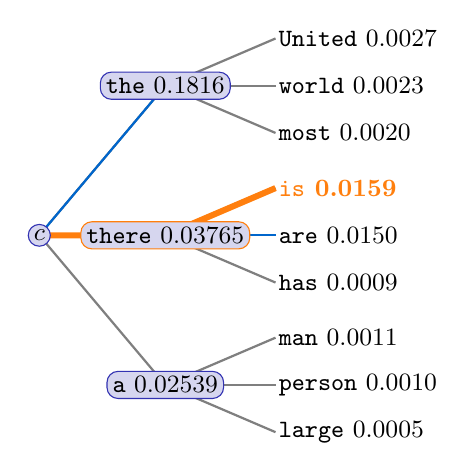
\begin{tikzpicture}[
  tk/.style={rectangle, rounded corners, draw=mlpurple, fill=mllavender4, font=\small, inner sep=2pt},
  lf/.style={font=\small, anchor=west, inner sep=1pt}]
  \coordinate (c) at (0, 0);
  \foreach \y in {1.9, 0, -1.9} \draw[thick, mlgray] (c) -- (1.6, \y);
  \foreach \y in {2.5, 1.9, 1.3} \draw[thick, mlgray] (1.6, 1.9) -- (3.0, \y);
  \foreach \y in {0.6, 0, -0.6} \draw[thick, mlgray] (1.6, 0) -- (3.0, \y);
  \foreach \y in {-1.3, -1.9, -2.5} \draw[thick, mlgray] (1.6, -1.9) -- (3.0, \y);
  \draw[thick, mlblue] (c) -- (1.6, 1.9);
  \draw[thick, mlblue] (1.6, 0) -- (3.0, 0);
  \draw[mlorange, line width=2.2pt] (c) -- (1.6, 0) -- (3.0, 0.6);
  \node[tk] at (c) {$c$};
  \node[tk] at (1.6, 1.9) {\texttt{the} 0.1816};
  \node[tk, draw=mlorange] at (1.6, 0) {\texttt{there} 0.03765};
  \node[tk] at (1.6, -1.9) {\texttt{a} 0.02539};
  \node[lf] at (3.0, 2.5) {\texttt{United} 0.0027};
  \node[lf] at (3.0, 1.9) {\texttt{world} 0.0023};
  \node[lf] at (3.0, 1.3) {\texttt{most} 0.0020};
  \node[lf, text=mlorange] at (3.0, 0.6) {\textbf{\texttt{is} 0.0159}};
  \node[lf] at (3.0, 0) {\texttt{are} 0.0150};
  \node[lf] at (3.0, -0.6) {\texttt{has} 0.0009};
  \node[lf] at (3.0, -1.3) {\texttt{man} 0.0011};
  \node[lf] at (3.0, -1.9) {\texttt{person} 0.0010};
  \node[lf] at (3.0, -2.5) {\texttt{large} 0.0005};
\end{tikzpicture}
\end{center}
{\small Leaves: $P$; blue: kept at $B = 2$; orange: the result.}
\end{columns}

\bottomnote{With $B = 2$, the result is \texttt{there is}, 5.9 times as probable as the greedy path \texttt{the United}.}
\note{2 min. Walk through $B = 2$: after step 1, \texttt{the} and \texttt{there} are kept; of their extensions, \texttt{there is} and \texttt{there are} are the two largest. In the tree, the condition of part 5 holds with $a$ = the, $b$ = there, $y$ = is: $0.0159 > 0.0027$. After \texttt{the}, the likeliest second token has 0.01472.}
\end{frame}

% ==================== WORKED NUMBERS: LOOP ====================
\begin{frame}[t]{Six Copies of One Sentence Under Greedy Decoding}
\begin{columns}[T]
\column{0.48\textwidth}
\begin{block}{Definition}
A \textbf{copy} is one occurrence of the sentence \textit{The United States is a nation of immigrants.} in the greedy continuation of the Austen prompt. Its probability $P$ is the product of its 9 token probabilities.
\end{block}

\vspace{1mm}
\begin{tabular}{lll}
\toprule
Copy & Tokens & $P$ \\
\midrule
1 & 1 to 9 & $5.268 \times 10^{-7}$ \\
2 & 10 to 18 & $3.812 \times 10^{-5}$ \\
3 & 19 to 27 & 0.01216 \\
4 & 28 to 36 & 0.1263 \\
5 & 37 to 45 & 0.3692 \\
6 & 46 to 54 & 0.6087 \\
\bottomrule
\end{tabular}

\vspace{1mm}
\textbf{Worked:} from copy 1 to copy 6, $P$ grows by $0.6087 / (5.268 \times 10^{-7}) = 1.16 \times 10^{6}$.

\column{0.48\textwidth}
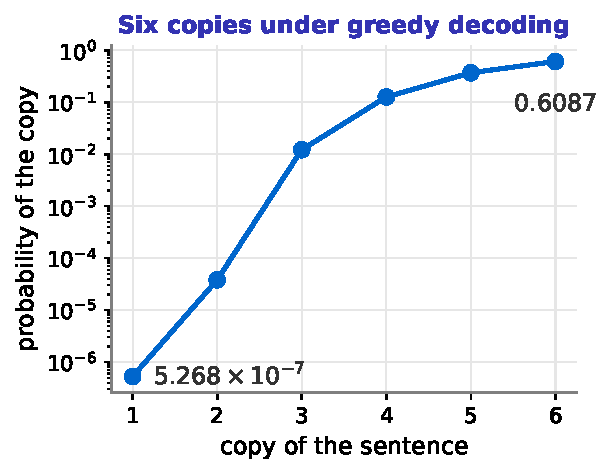
\includegraphics[width=\textwidth]{images/loop_copies.pdf}
\end{columns}

\bottomnote{Under greedy decoding, the probability of the sentence grows with every copy, from $5.268 \times 10^{-7}$ to 0.6087.}
\note{1.5 min. Copy 1 starts with lowercase \texttt{the}, at probability 0.182; from copy 2 on, with \texttt{The}. In copy 6, the first token has probability 0.649. This is the rise of the discovery on the repeated phrase, measured after one prompt.}
\end{frame}

% ==================== WORKED: TEXTS ====================
\begin{frame}[t]{Twenty Tokens After the Austen Prompt Under Five Rules}
Five rules, 20 tokens each after the Austen prompt; $\log P$ is the sum of the 20 log-probabilities of GPT-2 small at $T = 1$.

\vspace{2mm}
\small
\begin{tabular}{lrp{10.6cm}}
\toprule
Rule & $\log P$ & Continuation \\
\midrule
greedy, $B = 1$ & $-27.77$ & the United States is a nation of immigrants. The United States is a nation of immigrants. The United \\
beam, $B = 2$ & $-27.78$ & there is no such thing as a `good' or `bad' person. $\hookleftarrow\hookleftarrow$ It is \\
beam, $B = 5$ & $-25.14$ & there is no such thing as a ``right'' or ``wrong'' way of life. It is \\
$T = 0.7$, draw 0 & $-61.53$ & the best and the brightest minds in the world face incredible pain and surmounting adversity. The best \\
$T = 1.5$, draw 0 & $-169.60$ & WWI and the 1914 Ottoman Imperial Question originally parted rows) Leatherwolves moreapa hamley ancient \\
\bottomrule
\end{tabular}

\normalsize
\bottomnote{Over 20 tokens, $\log P$ is $-25.14$ under beam search of width 5 and $-169.60$ for a draw at $T = 1.5$.}
\note{1.5 min. Read the $\log P$ column from top to bottom. Beam search at $B = 2$ ends 0.01 below greedy decoding: the second checkpoint question. Another draw at $T = 0.7$ or $1.5$ gives another text; the three search texts are the same on every run.}
\end{frame}

% ==================== PYTHON CODE ====================
\begin{frame}[fragile,t]{\texttt{next\_token\_dist} on the Flat Prompt}
\begin{columns}[T]
\column{0.52\textwidth}
\begin{lstlisting}[language=Python]
z = logits("I went to the")             # 50,257 scores
p = next_token_dist(z, T=1.0)            # T = 1: GPT-2's p, no draw
q = next_token_dist(z, T=1.0, k=5)       # top-k, k = 5
r = next_token_dist(z, T=1.0, top_p=0.9) # top-p, pi = 0.9
print(word(p.argmax()), p.max())         # hospital 0.0331
print((q > 0).sum(), q.max())            # 5 0.2950
print((r > 0).sum())                     # 4797
\end{lstlisting}

\column{0.44\textwidth}
\textbf{Key outputs:}
\begin{itemize}\compactlist
\item \texttt{p.max()}: 0.0331, the probability of \texttt{hospital}
\item \texttt{q}: 5 tokens kept, \texttt{hospital} at 0.2950
\item \texttt{r}: 4,797 tokens kept at $\pi = 0.9$
\end{itemize}

\vspace{2mm}
\textbf{Note:} $0.0331 / 0.1122 = 0.2950$, the value of top-5 after the flat prompt.
\end{columns}

\bottomnote{Temperature, top-k, top-p are arguments of one function, \texttt{next\_token\_dist}.}
\note{1.5 min. The function is in the setup cell of the three notebooks. At $T = 1$ no token is drawn: the function gives the distribution. The order of the cuts is that of Hugging Face transformers: temperature, top-k, top-p, min-p.}
\end{frame}

% ==================== EXERCISE ====================
\begin{frame}[fragile,t]{Nucleus Size at Four Temperatures}
\begin{block}{Discovery Exercise}
Open \href{\colab{01_sampling_visual}}{\textbf{notebook 01}} in Colab, run the setup cell, then the four lines, at four temperatures:
\end{block}

\vspace{1mm}
\begin{lstlisting}[language=Python]
z = logits(AUSTEN)
for T in [0.5, 0.7, 1.0, 1.5]:           # four distributions, no draw
    r = next_token_dist(z, T=T, top_p=0.9)
    print(T, (r > 0).sum(), round(r.max(), 3))
\end{lstlisting}

\vspace{2mm}
\textbf{Questions to answer:}
\begin{enumerate}\compactlist
\item What is the size of the nucleus of 0.9 at each $T$?
\item What is the probability of \texttt{the} after the cut at $T = 0.5$, against 0.885 before it?
\item In \href{\colab{03_beam_search}}{\textbf{notebook 03}}, what is the smallest width $B$ with the result \texttt{there is}?
\end{enumerate}

\vspace{1mm}
Derivations with checks on GPT-2 small: \href{\colab{02_sampling_mathematics}}{\textbf{notebook 02}}.

\bottomnote{After the Austen prompt, the nucleus of 0.9 grows with the temperature.}
\note{1.5 min. Answers: 2, 42, 3,784, 15,670 tokens; 0.959, the share of \texttt{the} in the two kept tokens, $0.885 / (0.885 + 0.038) = 0.959$; $B = 2$. In notebook 02, the appendix formulas are checked on the scores of GPT-2 small.}
\end{frame}

% ==================== TAKEAWAYS ====================
\begin{frame}[t]{Five Results on Decoding the Next Token}
\begin{columns}[T]
\column{0.48\textwidth}
\textbf{Five results on decoding:}
\begin{enumerate}\compactlist
\item Softmax: $p_i = e^{z_i} / \sum_j e^{z_j}$; $P$ of a continuation is a product
\item Greedy decoding: $\arg\max_i p_i$; the probability of a repeated phrase grows with each copy
\item $p^{(T)} \propto e^{z / T}$: greedy decoding at $T \to 0$, uniform at $T \to \infty$
\item Top-$k$: $k$ tokens fixed; top-$p$: the mass $\pi$ fixed
\item Beam search: $B$ paths kept, $B = 1$ greedy; a wider beam can end on a smaller $\log P$
\end{enumerate}

\column{0.48\textwidth}
\begin{center}
\decodingdiagram
\end{center}
\end{columns}

\bottomnote{Each of the five rules is a map from one distribution per step to the next token.}
\note{2 min. Ask, for each result, for the frame number in the footline of its first page: result 1 on frames 4, 5; result 2 on 8, 9; result 3 on 11, 12; result 4 on 15, 16; result 5 on 19 to 21. The numbers of GPT-2 small for results 2, 5 are on frames 28 to 30.}
\end{frame}

% ==================== CLOSING ====================
\begin{frame}[t]
\vspace*{10mm}
\begin{center}
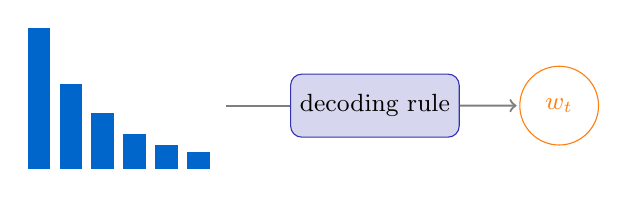
\begin{tikzpicture}[scale=0.9]
  \foreach \x/\h in {0/2.0, 0.45/1.2, 0.9/0.8, 1.35/0.5, 1.8/0.35, 2.25/0.25} \fill[mlblue] (\x, 0) rectangle (\x + 0.32, \h);
  \draw[->, thick, mlgray] (2.8, 0.9) -- (3.8, 0.9);
  \node[rectangle, rounded corners, draw=mlpurple, fill=mllavender4, font=\small, minimum height=0.8cm] (r) at (4.9, 0.9) {decoding rule};
  \draw[->, thick, mlgray] (r.east) -- (6.9, 0.9);
  \node[circle, draw=mlorange, fill=white, minimum size=1.0cm, font=\small\bfseries, text=mlorange] at (7.5, 0.9) {$w_t$};
\end{tikzpicture}

\vspace{4mm}
{\large\textbf{Thank you}}

\vspace{2mm}
Picking the Next Token\\
Text Analytics, Chapter 7
\end{center}
\end{frame}

% ==================== APPENDIX ====================
\appendix
\section{Appendix}

\begin{frame}[plain]
\begin{center}
\vspace{15mm}
\begin{beamercolorbox}[sep=8pt,center]{title}
\usebeamerfont{title}\textbf{Appendix}\\[4pt]
\small Derivations: entropy, truncation, min-p, repetition penalty
\end{beamercolorbox}
\end{center}
\end{frame}

\begin{frame}[t]{A2: Derivative of the Entropy in T}
% nouns: Derivative, Entropy
\textbf{Given} $p_i^{(T)} = e^{\beta z_i} / Z(\beta)$ with $\beta = 1/T$, $Z(\beta) = \sum_j e^{\beta z_j}$; expectations under $p^{(T)}$.

\vspace{3mm}
\textbf{Step 1:} $\log p_i = \beta z_i - \log Z$, so the entropy is
\[ H = -\sum_i p_i \log p_i = \log Z - \beta\, \mathbb{E}[z]. \]

\textbf{Step 2:} $\dfrac{d \log Z}{d\beta} = \mathbb{E}[z]$ and $\dfrac{d\, \mathbb{E}[z]}{d\beta} = \mathrm{Var}(z)$, so
\[ \frac{dH}{d\beta} = \mathbb{E}[z] - \mathbb{E}[z] - \beta\, \mathrm{Var}(z) = -\beta\, \mathrm{Var}(z). \]

\textbf{Step 3:} with $d\beta / dT = -1/T^2$, the derivative in $T$ is
\[ \frac{dH}{dT} = \frac{\mathrm{Var}_{p^{(T)}}(z)}{T^3} \ \ge\ 0. \]

\bottomnote{The entropy of $p^{(T)}$ grows with $T$ at the rate $\mathrm{Var}(z) / T^3$.}
\note{1.5 min. The variance is zero only when all scores are equal, and then $H = \log |V|$ at every $T$. In notebook 02, section 2, the formula is checked on the scores of GPT-2 small.}
\end{frame}

\begin{frame}[t]{A3: Divergence of a Truncation}
% nouns: Divergence, Truncation
\textbf{Given} a kept set $S$ with mass $M = \sum_{i \in S} p_i$; $q_i = p_i / M$ on $S$, $q_i = 0$ elsewhere. Top-$k$, top-$p$, min-$p$ are truncations of this form.

\vspace{3mm}
\textbf{Step 1:} on $S$, $q_i / p_i = 1/M$, so
\[ \mathrm{KL}(q \parallel p) = \sum_{i \in S} q_i \log \frac{q_i}{p_i} = \log \frac{1}{M} \sum_{i \in S} q_i = -\log M. \]

\textbf{Step 2:} under top-$p$, $M \ge \pi$, so $\mathrm{KL}(q \parallel p) \le -\log \pi$ after every prompt.

\vspace{2mm}
\textbf{Step 3:} under top-$k$, the $k$ largest of $|V|$ probabilities have a mean of at least $1/|V|$, so $M_k \ge k / |V|$ and $\mathrm{KL}(q \parallel p) \le \log (|V| / k)$.

\bottomnote{The divergence of a truncation is $-\log M$; it depends on the kept mass alone.}
\note{1.5 min. The total variation distance is $1 - M$ by the same steps. In the other direction, $\mathrm{KL}(p \parallel q)$ is infinite for $M < 1$: $p$ has mass on tokens with $q_i = 0$.}
\end{frame}

\begin{frame}[t]{A4: Bound on the Number of Tokens Under Min-p}
% nouns: Bound, Number, Tokens, Min-p
\begin{block}{Definition}
Under \textbf{min-p} (Nguyen et al., 2024), the kept set is $S = \{\, i : p_i \ge p_{\text{base}}\, p_{\max} \,\}$, with $0 < p_{\text{base}} < 1$.
\end{block}

\vspace{2mm}
\textbf{Step 1:} each kept token other than the likeliest has $p_i \ge p_{\text{base}}\, p_{\max}$; together these tokens have a mass of at most $1 - p_{\max}$.

\vspace{2mm}
\textbf{Step 2:}
\[ (|S| - 1)\, p_{\text{base}}\, p_{\max} \le 1 - p_{\max} \ \Rightarrow\ |S| \le 1 + \frac{1 - p_{\max}}{p_{\text{base}}\, p_{\max}}. \]

\textbf{Interpretation:} a peaked $p$, with $p_{\max}$ near 1 $\rightarrow$ few tokens; a flat $p$ $\rightarrow$ the bound grows as $1 / p_{\max}$.

\bottomnote{Under min-$p$, the number of kept tokens is at most $1 + (1 - p_{\max}) / (p_{\text{base}}\, p_{\max})$.}
\note{1.5 min. Min-p is a cut relative to the largest probability. With temperature first, the threshold on the scores is $z_i \ge z_{\max} + T \log p_{\text{base}}$, and the kept set grows with $T$. Nguyen et al. recommend $p_{\text{base}}$ between 0.05 and 0.1.}
\end{frame}

\begin{frame}[t]{A5: Repetition Penalty, Offset of the Scores}
% nouns: Repetition, Penalty, Offset, Scores
\begin{block}{Definition}
Under the \textbf{repetition penalty} $\theta > 1$ (Keskar et al., 2019), the score of each token already in the text is changed to
\[ z_i' = \begin{cases} z_i / \theta, & z_i > 0, \\ \theta\, z_i, & z_i \le 0. \end{cases} \]
\end{block}

\vspace{2mm}
\textbf{Step 1:} $\mathrm{softmax}(z + a) = \mathrm{softmax}(z)$ for every constant $a$: $p$ is the same at every offset of the scores.

\vspace{2mm}
\textbf{Step 2:} the penalty depends on the offset: for $z_i < 0$, the score falls by $(\theta - 1)\,|z_i|$, a fall that grows with $|z_i|$.

\vspace{2mm}
\textbf{Interpretation:} two score vectors with one softmax $p$ can give two different distributions after the penalty.

\bottomnote{The repetition penalty depends on the offset of the scores; the softmax is the same at every offset.}
\note{1.5 min. In Hugging Face transformers, negative scores are multiplied by $\theta$, since a division would raise them. After the Austen prompt, the scores of GPT-2 small lie between $-119$ and $-88$: the penalty is $\theta z_i$ for every token.}
\end{frame}

\end{document}
